\documentclass[main.tex]{subfiles}
\pgfplotsset{compat=1.18}

\begin{document}
    
    \chapter{Fiscal Policy}
       
    \section{Government Budget Constraint}
        Government's budget constraint is
        \begin{align}
            \int_{t=0}^\infty e^{-R(t)} G(t) dt 
            \le
            - D(0) + \int_{t=0}^\infty e^{-R(t)} T(t) dt
            \label{eqn:gov-budget}
        \end{align}
        
        where $G(t)$ is government spending, $T(t)$ is tax income, and government debt $D(t)$ follows law of motion:
        \begin{align}
            \dot D(t) = G(t) - T(t) + r(t) D(t)
        \end{align}
        
        \section{Ricardian Equivalence and Household constraints}
        The representative household is faced with the RCK-model budget constraint with lump-sum taxes. Government debt is also passed to households. Then the household budget constraint is
        \begin{align}
            \int_{t=0}^\infty e^{-R(t)} C(t) dt 
            & \le
            K(0) + D(0) + 
            \int_{t=0}^\infty e^{-R(t)} W(t) dt
            -
            \int_{t=0}^\infty e^{-R(t)}  T(t) dt
            \\
            &=
            K(0) + 
            \int_{t=0}^\infty e^{-R(t)} W(t) dt
            -
            \int_{t=0}^\infty e^{-R(t)} G(t) dt
            \\
            &=
            K(0) + 
            \int_{t=0}^\infty e^{-R(t)} [W(t) - G(t)] dt,
        \end{align}
        
        where $C(t)$ is consumption, $W(t)$ is wage income, and $K(0)$ is initial capital. This budget constraint implies taxes $T(t)$ do not affect the household's optimization problem. Only government spending $G(t)$ affects the household behaviour, but not the financing of the spending (i.e. taxes). This result is called \textbf{Ricardian equivalence (RE)}. Reasons RE may not hold:
        \begin{itemize}
            \item
            \textbf{Infinite lifetimes:} Turnover in population (i.e. finite lived households budget constraint) may cause the math to break.
            
            \item
            \textbf{Permanent Income Hypothesis (PIH)} implies that household consumes the same amount every period adjusted for time and interest discounting, saving or borrowing as needed to reach optimal consumption level. But \textbf{liquidity constraints} (i.e. borrowing limit) and \textbf{precautionary savings} (i.e. household maintaining minimum savings level) will create period specific budget constraints which make timing of taxes matter.
            
            \item
            \textbf{Distortionary taxes} (e.g. sales tax on consumption, progressive income tax) instead of lump-sum taxes can change household consumption/labor choices.
            
        \end{itemize}
        
        
        \section{Tax Smoothing}
        
        Assume tax rates do have distortionary effects on consumer income, which in each period is
        \begin{align}
            \Gamma_t = Y_t f\left(\frac{T_t}{Y_t}\right),
            \quad
            f'(\cdot) > 0,  f''(\cdot) > 0
        \end{align}
        
        Assume government's objective is to minimize distortion subject to some required spending:
        \begin{align}
            \min_{T_t}
            \sum_{t=0}^\infty
            \frac{1}{(1+r)^t}
            Y_t f\left(\frac{T_t}{Y_t}\right)
            \quad s.t. \quad
            D(0) + \sum_{t=0}^\infty \frac{1}{(1+r)^t} G(t)
            \le
            \sum_{t=0}^\infty \frac{1}{(1+r)^t} T(t)
        \end{align}
        
        Formulate Lagrangian for minimization:
        \begin{align}
            \mathcal{L}
            &= \sum_{t=0}^\infty
            \frac{1}{(1+r)^t}
            Y_t f\left(\frac{T_t}{Y_t}\right)
            + \lambda \left(
            D(0) + \sum_{t=0}^\infty \frac{1}{(1+r)^t} G(t)
            - \sum_{t=0}^\infty \frac{1}{(1+r)^t} T(t)
            \right)
        \end{align}
        
        Then taking FOC with respect to $T(t)$ at some period $t$, we have:
        \begin{align}
            \frac{\partial \mathcal{L}}{\partial T_t}
            = 0
            &\implies
            \frac{1}{(1+r)^t}
            Y_t f'\left(\frac{T_t}{Y_t}\right) \frac{1}{Y_t} = - \lambda \frac{1}{(1+r)^t}
            \\
            &\implies
            f'\left(\frac{T_t}{Y_t}\right)
            = \lambda
            % \implies
            % \frac{f'\left(\frac{T_t}{Y_t}\right)}{f'\left(\frac{T_{t+1}}{Y_{t+1}}\right)}
            % =\frac{\lambda}{\lambda} = 1
            \\
            &\implies
            f'\left(\frac{T_t}{Y_t}\right)
            = f'\left(\frac{T_{t+1}}{Y_{t+1}}\right)
            \implies
            \frac{T_t}{Y_t} = \frac{T_{t+1}}{Y_{t+1}},
        \end{align}
        implying optimal to impose same tax rate across all periods \textbf{(tax smoothing)}. 
    
    
    \section{Government Debt Crisis}
        
        Government pays interest factor $R = (1+r)$ on debt $D$, financed by taxes $T$. Assume $T$ is uniformly distributed in an interval:
        \begin{align}
            T \sim \text{Uniform}\left(\mu - X, \mu + X\right), \quad X, \; \mu - X \ge 0
        \end{align}
        
        Let $\pi$ be the probability the government defaults on its debt, which is occurs if $T < RD$.
        
        Then probability of default is
        \begin{align}
            \pi = P(T < RD)
            = \begin{cases}
                0
                & R < \frac{\mu-X}{D}
                \\
                \frac{RD - (\mu - X)}{2X}
                & R \in \left[
                    \frac{\mu-X}{D}, \frac{\mu+X}{D}
                    \right]
                \\
                1
                & R > \frac{\mu + X}{D}
            \end{cases}
            \label{eqn:tax-cdf}
        \end{align}
        where $T$ is the tax income, $F(\cdot)$ is the cumulative distribution function. \\
        
        If in default, government pays nothing. Assume investors are risk-neutral, and indifferent between expected return and risk-free factor $\bar{R}$, then
        \begin{align}
            0 \cdot \pi + R \cdot (1-\pi) = \bar R
            \implies
            \pi &= \frac{R - \bar R}{R}.
            \label{eqn:investor-indifference}
        \end{align}
        
            
        In equilibrium, interest and default probabilities $(R, \pi)$ are where
        \begin{align}
            \frac{R - \bar R}{R} = P(T < RD).
            \label{eqn:default-interest-eqm}
        \end{align}
        
        Illustrate examples of equilibria in Figure \eqref{fig:default-interest-eqm} with
        \begin{align}
            \mu = 2, \quad
            X = 0.95, \quad
            \bar R = 1.1, \quad
            D = 1.
        \end{align}
        
        \begin{figure}[H]
            \centering
            
            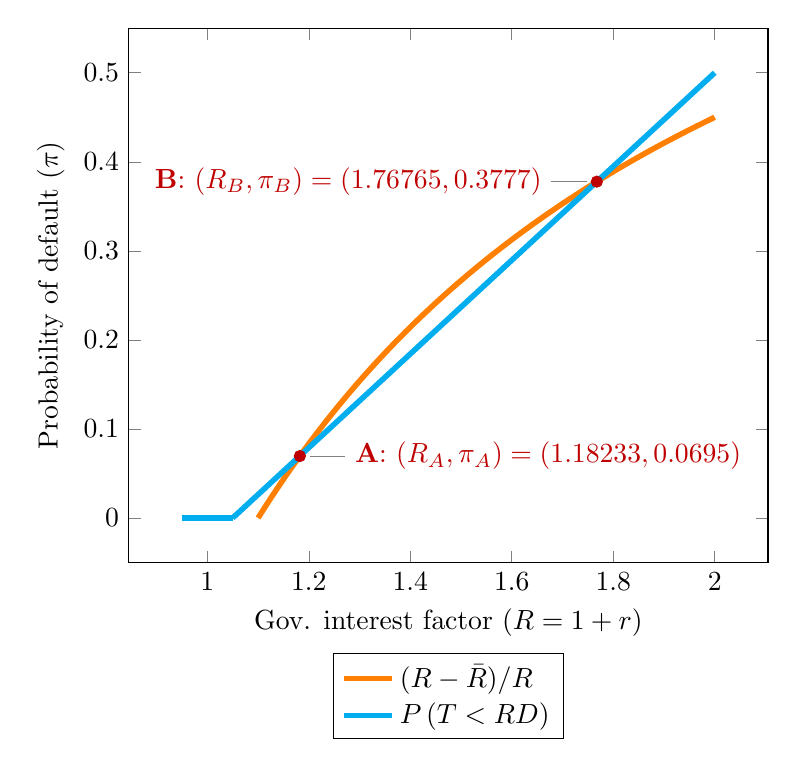
\begin{tikzpicture}
                \begin{axis}[
                    xlabel = {Gov. interest factor (\(R = 1+r\))},
                    ylabel = {Probability of default (\(\pi\))},
                    legend style={at={(0.5,-0.17)},anchor=north,legend cell align=left},
                    width = 0.8*\textwidth
                    ]
                    
                    % variables
                    \pgfmathsetmacro{\mu}{2}
                    \pgfmathsetmacro{\X}{0.95}
                    
                    \pgfmathsetmacro{\barR}{1.1}
                    \pgfmathsetmacro{\D}{1}
                    
                    \pgfmathsetmacro{\cdfbeg}{(\mu-\X)/\D}
                    \pgfmathsetmacro{\cdfend}{2}%{(\mu+\X)/\D}
                    
                    % plot range formatting
                    \pgfmathsetmacro{\xbeg}{0.95}
                    \pgfmathsetmacro{\xend}{2}
                    \pgfmathsetmacro{\lw}{2}
                    
                    % equilibrium calculations
                    \pgfmathsetmacro{\RA}{
                    (\mu+\X - ((-\mu-\X)^2-8*\D*\X*\barR)^(1/2)) / (2*\D)
                    }
                    \pgfmathsetmacro{\RB}{
                    (\mu+\X + ((-\mu-\X)^2-8*\D*\X*\barR)^(1/2)) / (2*\D)
                    }
                    
                    \pgfmathsetmacro{\piA}{(\RA - \barR)/\RA}
                    \pgfmathsetmacro{\piB}{(\RB - \barR)/\RB}
                    
                    % plot investor curve
                    \addplot[domain=\barR:\xend, samples=100, color=orange, line width=\lw pt] {(x-\barR)/x}; \addlegendentry{\((R - \bar R) / R\)}
                
                    % plot CDF
                    \pgfmathsetmacro{\cdfcolor}{"cyan"}
                    \addplot[domain=\cdfbeg:\cdfend, samples=100, color=\cdfcolor, line width=\lw pt] {(x*\D-\mu+\X)/(2*\X)}; \addlegendentry{\(P\left(T < RD\right)\)}
                    
                    % plot CDF outside of bounds
                    \addplot[domain=\xbeg:\cdfbeg, samples=2, color=\cdfcolor, line width=\lw pt] {0};
                    % \addplot[domain=\cdfend:\xend, samples=2, color=\cdfcolor, line width=\lw pt] {1};
                    
                    
                    % equilibria points
                    \addplot[only marks, color=red!75!black, mark=*]
                    coordinates {(\RA, \piA)(\RB, \piB)}
                        node[pos=0, pin=right:{\textbf{A}: \((R_A, \pi_A) = (\RA, \piA)\)}]{}
                        node[pos=1, pin=left:{\textbf{B}: \((R_B, \pi_B) = (\RB, \piB)\)}]{};
                \end{axis}
            \end{tikzpicture}
            
            \caption{$(R, \pi)$ Equilibria}
            \label{fig:default-interest-eqm}
        \end{figure}
        
        A third equilibrium exists where $R \to \infty$ and $\pi = 1$, where the investor will not lend at any interest and the government defaults.
        
        \subsection*{Implications}
        \begin{itemize}
            
            \item
            Intersect \textbf{B} is an unstable equilibrium. If investor believes default probability is less than $\pi_B$, the interest factor needed for them to invest results in a lower default probability than they expect. Then they may reduce estimate of $\pi$, and repeat the process until converging to \textbf{A}. Similar process can occur if investor's expectation of $\pi$ is above $B$, which through updating will converge to $(R, \pi) = (\infty, 1)$.
            
            \item
            Large differences in fundamentals are not needed for large differences in outcomes. Firstly, due to the convergence mechanism from previous point, expectations about default probability alone can lead to different equilibria. Secondly, small changes in $\bar R$ or distribution parameters of tax $T$ can affect equilibria points dramatically.
            
            \item
            Defaults are unexpected, since equilibria are always much less than 1 because of shape of the investor indifference curve.
            
            
        \end{itemize}
        
        
        
    
\end{document}